\subsection{LoginSignupStack}
Der \textbf{LoginSignupStack} besteht aus drei Screens:

\subsubsection{LoginScreen}
Im \textbf{LoginScreen} wird der Benutzer dazu aufgefordert, seine Anmeldedaten einzugeben.

\begin{figure}[H]
  \begin{center}
    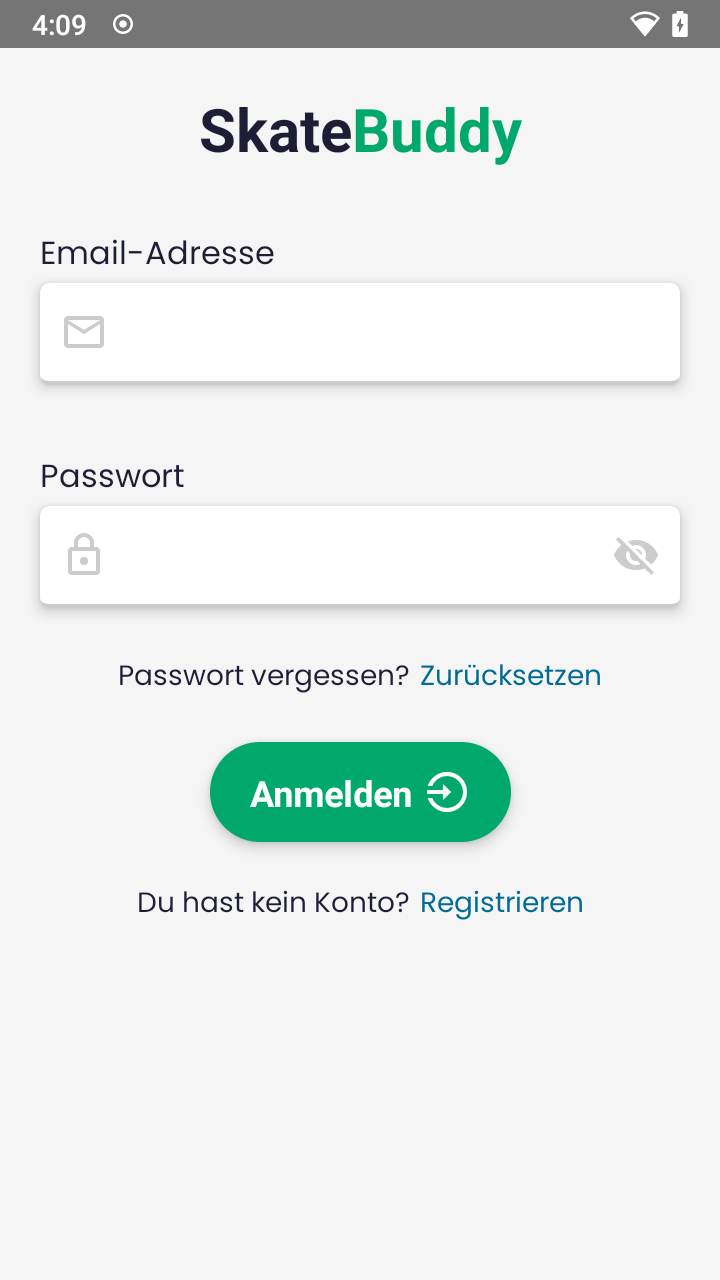
\includegraphics[width=0.6\textwidth]{Mobile/Login/Login.png}
    \caption{Daten eintragen und absenden.}
  \end{center}
\end{figure}

\subsubsection{SignupScreen}
Sollte er noch keinen Account haben, ist es ihm möglich, einen neuen Account zu erstellen über den
\textbf{SignupScreen}.

\begin{figure}[H]
  \begin{center}
    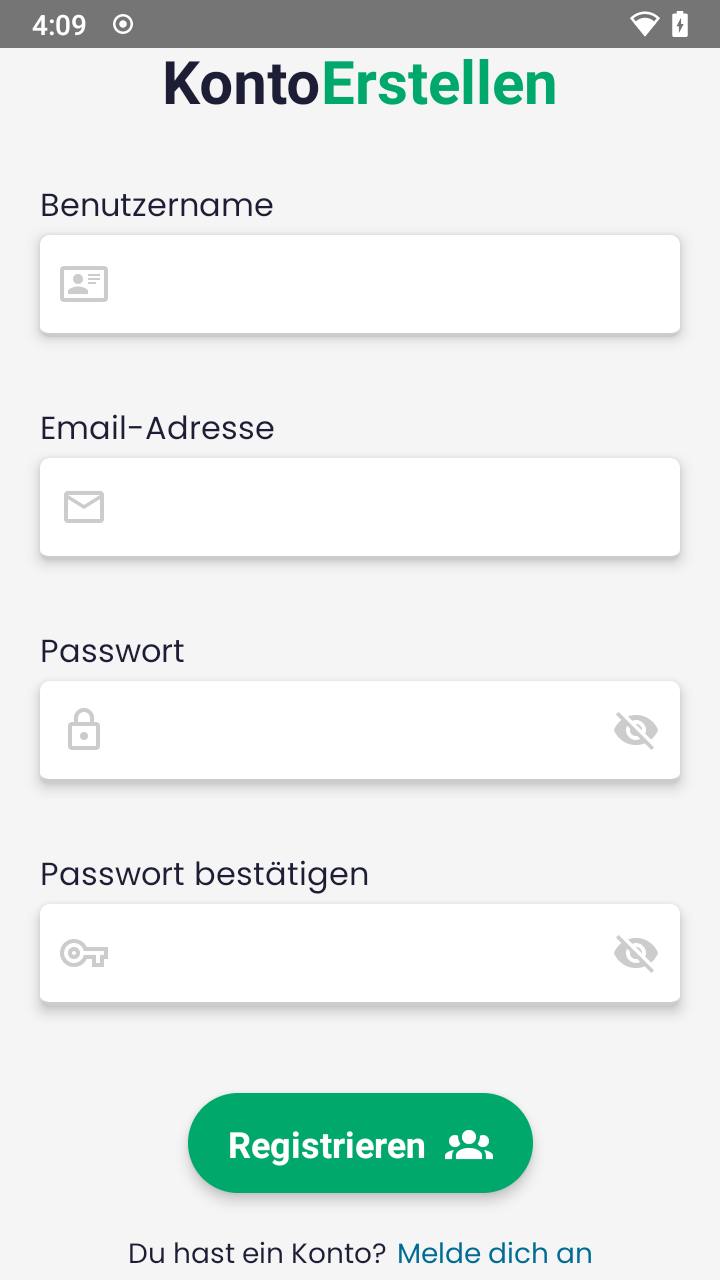
\includegraphics[width=0.6\textwidth]{Mobile/Login/Register.png}
    \caption{Daten eintragen und absenden.}
  \end{center}
\end{figure}

\subsubsection{ForgotPassword}
Wenn es dem Benutzer passieren sollte, dass er sein Passwort vergisst und keinen Zugriff auf seinen
Account mehr hat, so kann er über diesen Bildschirm einen Link anfordern, mit dem er sein Passwort
zurücksetzen kann. Dieser Link wird per E-Mail versendet.

Diese Funktion ist noch nicht in unserer App vorhanden, bis jetzt wird einfach überprüft, ob diese
E-Mail-Adresse existiert.

\begin{figure}[H]
  \begin{center}
    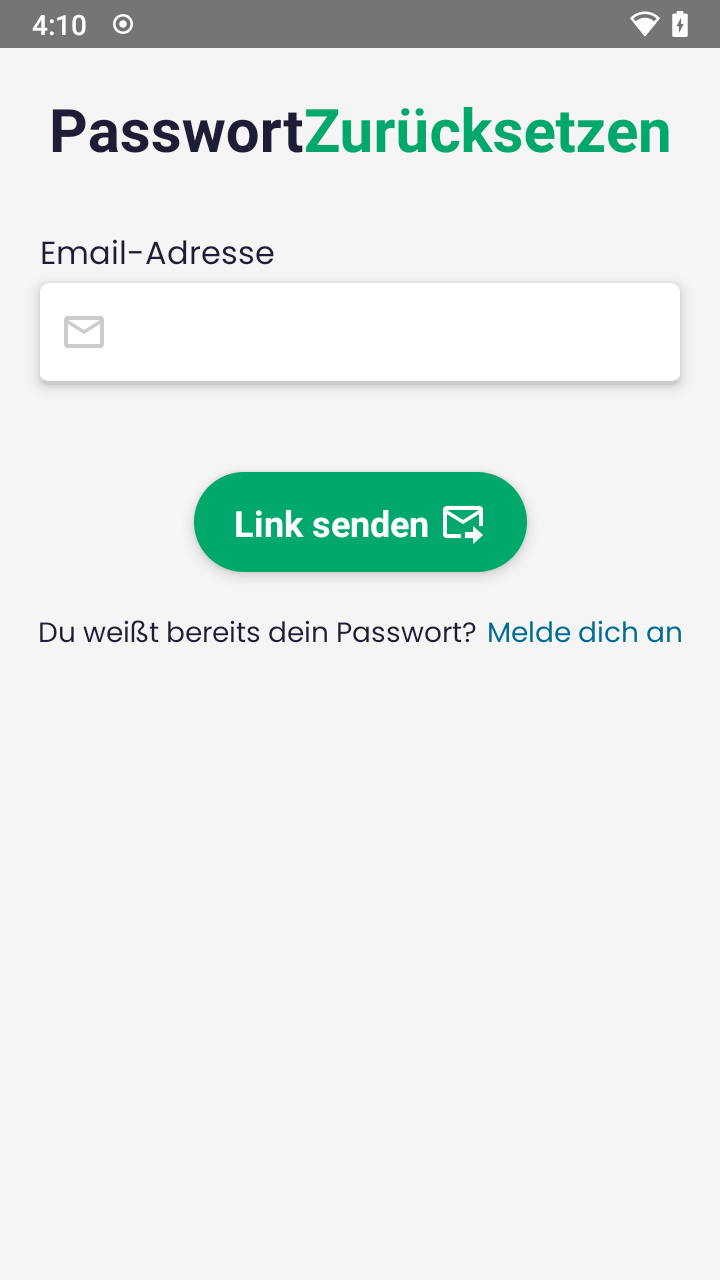
\includegraphics[width=0.6\textwidth]{Mobile/Login/Forgot.png}
    \caption{Daten eintragen und absenden.}
  \end{center}
\end{figure}
